\begin{figure}
  \centering
  \vskip -0.25cm
  \begin{tikzpicture}
    \node at (0, 0){
      \includegraphics[width=5cm]{experiments/2d/ppca_occ_ml/easy_5/results}
    };
    \node at (0, -4){
      \includegraphics[width=5cm]{experiments/2d/vae_occ_ml/easy_5/results_only}
    };
    \node at (0, -6.5){
      \includegraphics[width=5cm]{experiments/2d/ppca_occ_dl/easy_5_df/results_only}
    };
    \node at (0, -9){
      \includegraphics[width=5cm]{experiments/2d/vae_occ_dl/easy_5_df/results_only}
    };
    
    \draw[-,dashed] (2.75, -10.25) -- (2.75,3);
    
    \node at (5.5, 0){
      \includegraphics[width=5cm]{experiments/2d/ppca_occ_ml/hard_5/results}
    };
    \node at (5.5, -4){
      \includegraphics[width=5cm]{experiments/2d/vae_occ_ml/hard_5/results_only}
    };
    \node at (5.5, -6.5){
      \includegraphics[width=5cm]{experiments/2d/ppca_occ_dl/easy_5_df/results_only}
    };
    \node at (5.5, -9){
      \includegraphics[width=5cm]{experiments/2d/vae_occ_dl/easy_5_df/results_only}
    };
    
    \node at (8.5,0) {
      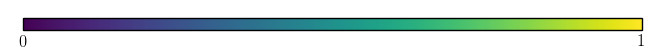
\includegraphics[height=5.5cm]{experiments/2d/vae_occ/colorbar}
    };
    
    \node[rotate=90] at (-3,-1.5) {\ML \PPCA};
    \node[rotate=90] at (-3,-4) {\ML \VAE};
    \draw[-,dashed] (-3,-2.75) -- (8.5,-2.75);
   
    \node[rotate=90] at (-3,-6.5) {\DL \PPCA};
    \draw[-,dashed] (-3,-5.25) -- (8.5,-5.25);
   
    \node[rotate=90] at (-3,-9) {\DL \VAE};
    
    \node at (0, 3) {\easy};
    \node at (5.5, 3) {\hard};
  \end{tikzpicture}
  
  % TODO short caption
  \caption{Qualitative results for \ML and \DL using both \PPCA and \VAE priors.
  We show results for the \easy and the \hard cases in the respective columns.
  For each approach, we show five shape predictions including the corresponding
  error. On top we additionally show the observed points, the free space as well
  as the target shape.}
  \label{fig:experiments-2d-ml-qual}
\end{figure}
